In order to check for security vulnerabilities we first have to find a suitable way to represent a program. This representation has to contain specific information about the program to be able to answer questions about security vulnerabilities. The information we need in this dissertation is twofold:

\begin{enumerate}
\item A program can contain many branches, loops and other control structures. We need to know the exact order of execution along each path in the program before we can make assumptions about security vulnerabilities. Therefore information is needed about which functions can be applied at a call site. This type of information is called \textit{control flow}.
\item Variables in JavaScript are mutable, so their values can change at any moment in a program. \textit{Value flow} information tells us exactly what values an expression may evaluate to. This is very important w.r.t. security, as some harmless variable may become referenced to a malicious variable somewhere in the program. From there on, that variable should be marked as pointing to the same value as the malicious variable.
\end{enumerate}

Aside from the representation, some technique has to be found to efficiently express security checks in the form of user-specified, application specific security policies. A naive way to examine programs would be to run them and keep track of any relevant information along the execution. Not only would this be tiresome, we can also not guarantee that the program will ever terminate, that it terminates without errors, or that it will have the same outcome for different inputs. A better approach would be to to analyze the program without having to run it. To this extent, a technique called \textit{static analysis} can be used.

This chapter describes how static analysis can be used to examine programs and how this analysis can be addressed to obtain information about specific parts of a program. First, section \ref{sec:staticAnalysis} describes more precisely what static analysis is and how it is interesting for this dissertation. Next, We discuss some approaches using static analysis to find generic vulnerabilities in programs in section \ref{sec:genericVulnerabilities}. Finally, some application-specific approaches for checking security vulnerabilities are discussed. For these approaches we take a deeper look on how they query the information specified by the analyses they perform. We end this chapter by giving a brief conclusion.

\section{Introduction to static analysis}
\label{sec:staticAnalysis}
Rice's theorem tells us that there is no general or effective method to prove non-trivial properties about a program. This problem is similar to the halting problem, which is undecidable. \textit{Static analysis} is a technique for analyzing computer programs without having to execute them. In this way we can avoid the possible problems we might encounter using a naive technique, as described above. The results of the analysis indicate program defects or prove certain properties of the program. As proving non-trivial properties about a program is undecidable, static analysis focusses on the instances of the problem about which it can tell whether the program satisfies a property or not, and leaves other instances unsolved. The results of the static analysis will then be a useful set of approximate solutions. Figure \ref{fig:decider} shows the main difference between a regular decider, which will always provide an exact answser, and a static analyzer.

\begin{figure}[!h]
    \centering
      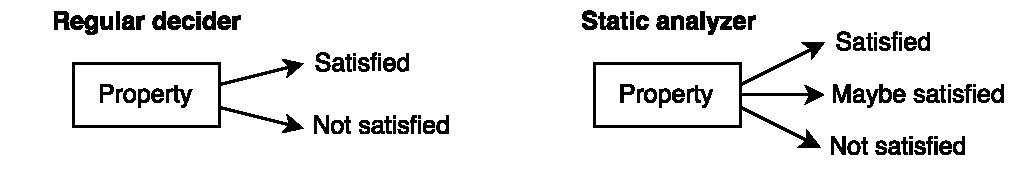
\includegraphics[width=0.9\textwidth]{images/decider} 
      \caption{Proving program properties: Regular decider and static analyzer}
    \label{fig:decider}
\end{figure}

\textit{Precision} is very important in static analysis. Consider a static analyzer that concludes for each property that it is \textit{maybe} satisfied. It is clear to see that there is no precision in this analysis, rendering it useless. We have to strive to attain enough precision to solve the maximum number of problem instances. \textit{Speed} on the other hand is less important for static analysis. As static analysis is decidable, it is guaranteed that the analysis will run in finite time, but gathering precise results is much more meaningful than the performance of the analysis itself. 
One particularly interesting technique used for static analysis is \textit{abstract interpretation}. This technique mimics interpretation of the program and allows to stay close to the original language semantics of those program without having to modify or instrument them to perform the analysis (in contrast to other static analysis techniques such as \textit{symbolic execution}). This mimicing of programs fits well for this dissertation, as we need to check for application-specific security vulnerabilities. It is thus a prerequisite that the semantics of the analyzed program lean as close to the original semantics as possible. A nice feature of abstract interpretation is that it allows to specify the precision needed by parameterizing it with e.g. a \textit{lattice}.

\subsection{Abstract interpretation}
%Quentin thesis
Abstract interpretation is a static analysis technique used to reason about a program. It does this by interpreting an approximation of a program through abstraction of its semantics. A \textit{sound} analysis can be performed and the precision of this analysis can be adjusted to the user's needs through various mechanisms. This increase in precision comes at the cost of a greater analysis running time. 

Abstract interpretation works in a similar way as normal program interpretation (so-called \textit{concrete interpretation}). The concrete interpretation of a program can be described as follows: A program \textit{e} can be injected into an initial state \textit{$s_0$}, the entry point of the program. From this state other states can be reached using a \textit{transition function}, until after several transitions a final state is reached. If no such state is ever reached, the execution will not terminate and hence will run indefinitely. The output of interpreting a program like this is a possibly infinite trace of execution states. The layout of this execution trace might depend on the input of the program or other changing values, making it useless for static analysis. 

Abstract interpretation solves this by applying abstraction in order to compute a finite trace. Primitive values and addresses are \textit{abstracted} to be made finite, resulting in something which is computable in finite time but less precise. Abstract interpretation is similar to concrete interpretation: A program is again injected, but this time into an \textit{abstract state} $\hat{s_0}$. A transition from one state to another is done through an \textit{abstract transition function}. The difference between this and a regular transition function is that an abstract state can make an abstract transition to multiple states. This is a consequence of the precision loss due to abstraction. Figure \ref{fig:abstractInterpretation} shows the concrete and abstract interpretation traces for \texttt{while(x < 5)\{ x--;\}}. We assume that for the concrete case \texttt{x} is smaller than 5 when it reaches the code. The program will then never terminate, leading to an infinite execution trace. For the abstract case, we assume that \texttt{x} is abstracted. We see that in abstract state $\hat{s_3}$ the program can go to either $\hat{s_4}$ or $\hat{s_4}'$, and that the (possibly infinite) \texttt{while} loop is represented as a loop in the abstract state graph. This finite representation of a program (which is actually an abstract state graph) proves to be useful to provide answers to non-trivial questions about the program.

\begin{figure}[!h]
    \centering
      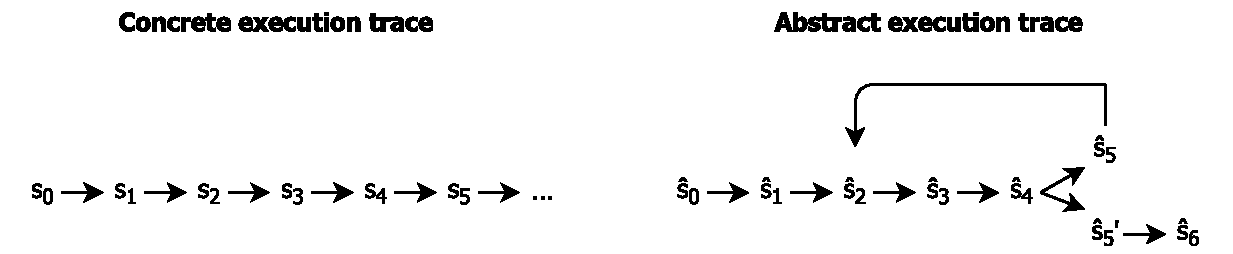
\includegraphics[width=1.0\textwidth]{images/abstractInterpretation} 
      \caption{Traces of concrete and abstract interpretation}
    \label{fig:abstractInterpretation}
\end{figure}


\subsection{Mathematical background}
\label{subsec:lattice}

In order to fully understand abstract interpretation, we will first look at the mathematical concepts it relies on. The concepts defined in this section will aid us in formally defining an \texttt{abstraction}. This definition is needed to understand how precision is caused by abstracting values.

\begin{definition}
\textit{A relation $\sqsubseteq: S \times S$ is a \textbf{partial order} if it has the following characteristics:}
\begin{enumerate}
\item Reflexivity: $\forall x \in S : x \sqsubseteq x$
\item Transitivity:  $\forall x,y,z \in S : x \sqsubseteq y \wedge y \sqsubseteq z \Rightarrow x \sqsubseteq z$
\item Anti-symmetry: $\forall x,y \in S : x \sqsubseteq y \wedge y \sqsubseteq x \Rightarrow x = y$
\end{enumerate}
\end{definition}
\begin{definition}
\textit{A \textbf{partially ordered set} ($S$,$\sqsubseteq$) is a set with a partial order}
\end{definition}
\begin{definition}
\textit{For a subset $X \subseteq S$, $u$ is an \textbf{upper bound} of $X$ if $u\in S, \forall x \in X: x \sqsubseteq u$. $u$ is the \textbf{least upper bound} of $X$ ($\bigsqcup X$) if for every upper bound $x$, $u \sqsubseteq x$. Similarly, the \textbf{lower bound} of $X$ can be defined as: $l \in S,\forall x \in X: l \sqsubseteq x$. $l$ is the \textbf{greatest lower bound} of $X$ ($\bigsqcap X$) if for every lower bound $x, x \sqsubseteq l$. Two important operators on partial orders are \textbf{join} ($\sqcup$) and \textbf{meet} ($\sqcap$). $x \sqcup y$ denotes $\bigsqcup\{x,y\}$, the least upper bound of $x$ and $y$, $x \sqcap y$ denotes $\bigsqcap\{x,y\}$, the greatest lower bound of $x$ and $y$.}
%Least upper bound
\end{definition}

\begin{definition}\label{def:lattice}
\textit{A \textbf{lattice} $(L,\sqsubseteq)$ is a partially ordered set in which any two elements have a least upper bound and a greatest lower bound. A \textbf{complete lattice} $(C,\sqsubseteq)$ is a partially ordered set in which all subsets have a least upper bound and a greatest upper bound. A complete lattice includes two special elements: a \textbf{bottom} element $\bot = \bigsqcap C$ and a \textbf{top} element $\top = \bigsqcup C$.}
\end{definition}

\begin{definition}
\textit{A \textbf{Galois connection} is a particular correspondence between two partially ordered sets $(A\sqsubseteq_A)$ and $(B\sqsubseteq_B)$. More precisely this correspondence is a pair of functions: the \textbf{abstraction function} $\alpha : A \rightarrow B$ and the \textbf{concretization function} $\gamma : B \rightarrow A$, such that $\forall a \in A, b \in B: \alpha(a) \sqsubseteq_B b \Leftrightarrow a \sqsubseteq_A \gamma(b)$.}
\end{definition}

%TODO: lattice voorbeeld
\begin{figure}
% center everything in the figure
\centering
% horizontal node distance
\begin{tikzpicture}[node distance=2cm]

\title{Partially ordered set of signs (complete lattice)}
\node(TOP)                          			 {$\top$};
\node(PLUS)     [below right=.6cm and .6cm of TOP] {$+$};
\node(ZERO)     [below=.6cm of TOP]       		 {$0$};
\node(MINUS)    [left=.6cm of ZERO]       		 {$-$};
\node(BOT)     	[below=1.8cm of TOP] {$\bot$};
\draw(TOP)      -- (PLUS);
\draw(TOP)      -- (ZERO);
\draw(TOP)      -- (MINUS);
\draw(BOT)      -- (PLUS);
\draw(BOT)      -- (ZERO);
\draw(BOT)      -- (MINUS);
\end{tikzpicture}
\caption{Partially ordered set of signs (complete lattice)}
\label{fig:lattice}
\end{figure}

\subsection{Abstraction}
An \textit{abstraction} $\hat{X}$ of a concrete set $X$ in abstract interpretation is a Galois connection between the power set of $X$ $(\mathcal{P}(X),\subseteq)$ and $X$ itself $(X,\sqsubseteq)$. The abstraction function $\alpha$ maps a concrete value to its abstract counterpart, whereas the concretization $\gamma$ function maps an abstract value to its concrete counterpart\textit{s}. Abstract values, sets and operations are generally indicated with a hat. The following abstraction example illustrates how abstraction works, and how it causes \textit{imprecision} to occur.\\\\
\textbf{Example} (Sign abstraction). A possible abstraction of integers $\mathbb{Z}$ could be to map them onto the set of signs $\widehat{Sign}$. The set of signs forms a complete lattice with $\sqsubseteq$ ordering, as depicted in figure \ref{fig:lattice}. This abstraction could be used in an analysis to detect divisions by zero, for example. We can define the abstract and concretization functions as follows:\\


\centerline{$\alpha:\mathcal{P}(\mathbb{Z}) \rightarrow \widehat{Sign}$}
\centerline{$\alpha(Z) = \bot$ when $Z = \varnothing$}
\begin{addmargin}[5.84cm]{1em}% 1em left, 2em right
$= 0$ when $Z = \{0\}$\\
$= +$ when $\forall z \in Z, z > 0$\\
$= -$ when $\forall z \in Z, z < 0$\\
$= \top$ otherwise
\end{addmargin}
\leavevmode \\\\
\centerline{$\gamma:\widehat{Sign} \rightarrow \mathcal{P}(\mathbb{Z})$}
\centerline{$\gamma(P) = \varnothing$ when $P = \bot$}
\begin{addmargin}[5.84cm]{1em}% 1em left, 2em right
$= {0}$ when $P = \hat{0}$\\
$= \mathbb{Z}^+$ when $P = +$\\
$= \mathbb{Z}^-$ when $P = -$\\
$= \mathbb{Z}$ otherwise\\
\end{addmargin}
\leavevmode \\
The addition operator $+$: $\mathbb{Z}\times\mathbb{Z}\rightarrow\mathbb{Z}$ can also be abstracted to $\hat{+}$: $\hat{\mathbb{Z}}\times\hat{\mathbb{Z}}\rightarrow\hat{\mathbb{Z}}$ following the rules of sign. Some examples:\\


\centerline{$\{0\}  \hat{+}  \{+\} = \{+\}$}
\centerline{$\{-\}  \hat{+}  \{-\} = \{-\}$}
\leavevmode \\
but for more advanced examples, we can easily see a loss in precision:\\\\
\centerline{$\{+\}  \hat{+}  \{-\} = \{-,0,+\}$}
\centerline{$\{0\}  \hat{+}  \{0,+\} = \{0,+\}$}
\\\\
When applying the concretization function after the abstraction function, we observe that the result is less precise. Consider the negation function $f(N) = \{-n \vert n \in N\}$, which negates an integer. Applying the concretization function to an integer directly results in no loss of precision:\\ 
\centerline{$f(\{1\}) = \{-1\}$,}\\ whereas applying it after the application of the abstraction function overapproximates the concrete value: \\
\centerline{$(\gamma \circ f \circ \alpha)(\{1\}) = \mathbb{Z}^+$}\\
$\mathbb{Z}^+$ is an overapproximation of $\{1\}$, conserving all properties that hold for $\{1\}$. The closer something is abstracted to its concrete value, the higher the precision of the analysis will be.

\subsection{conclusion}
To conclude this section, we briefly discuss why this loss of precision is important for this dissertation. When calculating value flow by performing static analysis through abstract interpretation, precision is also lost. In most programming languages, variables and objects point to values and addresses respectively. For this, JavaScript is no exception. It is obvious to see that simple calculations lose precision as in the example above. As a result of abstract interpretation, multiple addresses may point to the same object. This is exactly the kind of imprecision that is introduced in the analysis that is used in this dissertation. As each of these addresses is as valid of an address as any other, we need to consider all addresses of matched variables/objects on all matched paths in the state graph.

\section{Support for generic vulnerabilities}
\label{sec:genericVulnerabilities}

Static analysis is often used by model checkers to verify if a program satisfies a set of properties (i.e. a specification of a program). These tools often require additional information to be added to the program before being able to analyze it. The OWASP LAPSE+ plugin for Eclipse\cite{OWASP:LAPSE} for example requires the user to annotate all possible vulnerability sources and sinks in the source code. It then checks if there is information flow between a source and a sink. Although applicable to many programs, tools for finding general characteristics of programs is limited in several ways:
The set of problems that these tools can detect is often restricted and a lot of tools support detection for similar problems. Tools detecting bug patterns detect only the patterns that are pre-encoded in the tool. This implies that the tool only supports bug patterns that are pre-encoded and thus will most likely miss any bug pattern that isn't already encoded. Additionally, poorly encoded patterns may miss bugs, making the analysis of the tool unsound. Adding or extending functionality to existing solutions is often cumbersome and in most cases even impossible to do manually, which makes these solutions less useful for certain domain-specific programs, as these require a flexible tool. To this extent, a more practical approach would be to develop a tool which allows users to define by themselves what they wish to detect in a program. This approach would make the analysis \textit{application-specific} and the detection rules would be \textit{user-defined}. More about application-specific approaches can be found in section \ref{sec:applicationSpecificVulnerabilities}. The remainder of this section discusses the most popular static analysis approaches for model checking and finding generic code characteristics and vulnerabilities.

\subsection*{JOANA}
The Java Object-Sensitive Analysis project (JOANA\cite{JOANA}) is an eclipse plugin which checks for security leaks in Java programs. The tool supports all Java language features (except for reflection) and scales well for larger programs. The analysis they use is flow-sensitive, context-sensitive, object-sensitive and lock-sensitive, minimizing the amount of false positives drastically. The types of security flaws JOANA is able to detect are:
\begin{enumerate}
\item \textit{Confidentiality}: Information about sensitive values, like passwords or personal data, should in no case be conveyed to public outputs.
\item \textit{Integrity}: The dual of confidentiality: In no way should unsafe program inputs alter secure data or influence sensitive computations of a program.
\end{enumerate}
These flaws are detected by creating a system dependence graph (SDG) of the program on which information flow between sources and sinks is checked through program slicing. The SDG is an overapproximation of the information flow through the program. A benefit of this kind of graph is that it is able to detect direct (data dependencies) as well as indirect (control dependencies) dependencies. In order for the analysis to run, the user has to specify which parts of a program should act as sources and which should acts as sinks. This is done by adding annotations to the source code. JOANA comes with a machine-checked soundness proof. Although JOANA is good in what it does, it is limited in the amount of vulnerabilities it detects and there is no way to extend the tool to support more vulnerabilities.

\subsection*{Flawfinder}
%Flawfinder -> geen CF of DF
Flawfinder\cite{flawfinder} is a tool for examining C/C++ source code and detecting security weaknesses. It comes with a database of well-known problems, such as buffer overflow risks and race conditions. The results of the analysis performed is a report of all found flaws with a corresponding security risk level. Although being useful to quickly check for security vulnerabilities, flawfinder is not flexible as it is not extensible, nor is it aware of the semantics of the system under test. Control flow and data flow analysis aren't supported by the tool, making it rather a rather naive approach.

\subsection*{FindBugs}

FindBugs\cite{Findbugs} is a static analysis tool for detecting bugs in Java programs. They detect many classes of bugs by checking structural bug patterns against a program's source code. These classes of bugs can be subdivided into three main classes: Correctness bugs, dodgy confusing code and bad practices. Recently, the Find Security Bugs plugin\footnote{http://find-sec-bugs.github.io} was developed on top of Findbugs. This plugin can detect 80 different (pre-encoded) vulnerability types, among which are the top 10 OWASP security vulnerabilities. An example security violation detected by the plugin is the parsing of an untrusted XML file. The contents of this file might be malicious ant thus poses as a risk for the application. As the plugin is able to detect a wide range of bugs, it an ideal tool to checking for the most common security vulnerabilities. Nevertheless, only those vulnerabilities can be detected, and when a new class of security violations arises, there will be no way to add detection rules for them as a regular user.

%\subsection*{PMD}
%\footnote{https://pmd.github.io/}
%\subsection*{Splint}
%\cite{splint}
%http://www.cs.virginia.edu/~evans/pubs/ieeesoftware-abstract.html
%annotations

\subsection*{CodeSonar}
CodeSonar\cite{CodeSonar}, developed by GrammaTech, is a proprietary source code analysis tool that performs an unified data flow and symbolic execution analysis for C, C++ and Java programs. They claim to detect more code flaws than the average static analysis tool because they don't rely on pattern matching or other similar approximations. The approach they use is to compile source code and generate several intermediate representations, such as control flow graphs, call graphs and AST's. They then traverse/query these models to find particular properties or patterns that indicate defects. Next to performing general checks, CodeSonar provides an C API which gives access to its intermediate representations of the compiled program. A user can then define custom checks on these representations. We can't verify the ease of use of these custom checks as we couldn't find any examples. The hybrid approach of CodeSonar (general checks \textit{and} application-specified checks) preludes the next section of this chapter, which discusses approaches that support detecting application-specific vulnerabilities through user-defined queries and rules.


\section{Support for application-specific vulnerabilities}
\label{sec:applicationSpecificVulnerabilities}

The problem with tools supporting detection of generic vunerabilities is that they often don't allow users to write their own rule or queries to find domain- and/or application-specific flaws. Even if some mechanism for specifying user-defined rules is available, as in PMD\footnote{https://pmd.github.io} for example, it often is cumbersome to write them in the tool's input language. This limitation makes that these tools are often not very flexible, and it makes it hard to extend them. 

In this section we discuss how putting the detection of application-specific characteristics and vulnerabilities in the hands of the application developer can be fruitful, by presenting some approaches which allow users to define their own program queries. Two main considerations for creating such a tool are (i) the way a program is represented and (ii) how the user is given access to this representation. The following approaches each have their own techniques to do so, and we will elaborate on their advantages and disadvantages.


\subsection*{PQL}

The PQL language is designed to check if a program conforms certain program design rules\cite{PQL}. More precisely, it can be used to check the presence of sequences of events associated with a set of related objects. The language allows programmers to query for these types of sequences in an application-specific way, rendering very useful to detect design defects on a per application basis.

Either dynamic or static analysis can be used to solve these PQL queries, but only the latter is of interest for this dissertation. The static analyser described uses a context-sensitive, flow-insensitive, inclusion-based pointer analysis. As PQL attempts to optimize results of the static analysis to use them in the dynamic analysis, the used analysis must be sound. The points-to information, together with the program representation, is stored as datalog rules in a deductive database called \textit{bddbddb}. This is very similar to the approach of GateKeeper\cite{GateKeeper}.

%subqueries/reacting to a match
Two interesting features of the PQL language are the support for subqueries and the ability to react to a match. The latter is only useful in the case we use dynamic analysis. Subqueries however add significant power to a language. In the case of PQL, they allow users to specify recursive event sequences of recursive object relations. Figure \ref{fig:derivedStream} shows how a recursive query is written in the PQL language.

\begin{figure}[!ht]
    \centering
      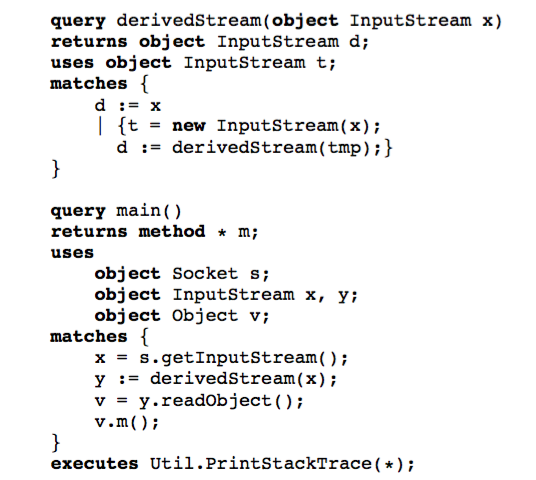
\includegraphics[width=0.5\textwidth]{images/derivedStream} 
      \caption{A PQL recursive query for tracking data from sockets}
    \label{fig:derivedStream}
\end{figure}

The actual matching of queries to these rules happens by first translating the PQL queries to the corresponding datalog queries. This happens automatically, to shield the user from dealing with the points-to information or the datalog program representation directly. Once translated, the queries get resolved by the \textit{bddbddb} system, after which te results are ready to be interpreted by the user. One thing to note is that since the analysis used is flow-insensitive, sequencing is not supported in such a way that the user can distinguish whether program point \texttt{a} happens before or after program point \texttt{b}. The same goes for negation: No guarantees about ordering can be made, which means that one can not deduce that an excluded event (i.e. a negated event) happens between two points in a sequence. They solve this by ignoring all excluded events, in order to maintain soundness of their approach.

A benefit of using Datalog is that it is very efficient and has way less overhead compared to fully fledged declarative programming languages. Storing an analysis/program as datalog rules may be efficient, but it is hard to get a good overview of the program by just looking at these rules. PQL closes the gap between the lack in readability of plain datalog rules and writing clean application-specific queries by introducing its own language. However, this language feels somewhat verbose and the syntax is something the user has to get used to.

\subsection*{Pidgin}

Pidgin\cite{PidginQL} is a program analysis and understanding tool which allows users to specify and enforce application-specific security guarantees. In their approach they generate a \textit{Program Dependence Graph} (PDG) of programs by using an interprocedural data flow analysis (object-sensitive pointer analysis). This kind of graph contains all information about how data data flows through a program. More precisely, each pair of connected nodes indicates that the second node of the pair depends in some way on the first node. Figure \ref{fig:PDG} shows a PDG of a guessing game.

\begin{figure}[!ht]
    \centering
      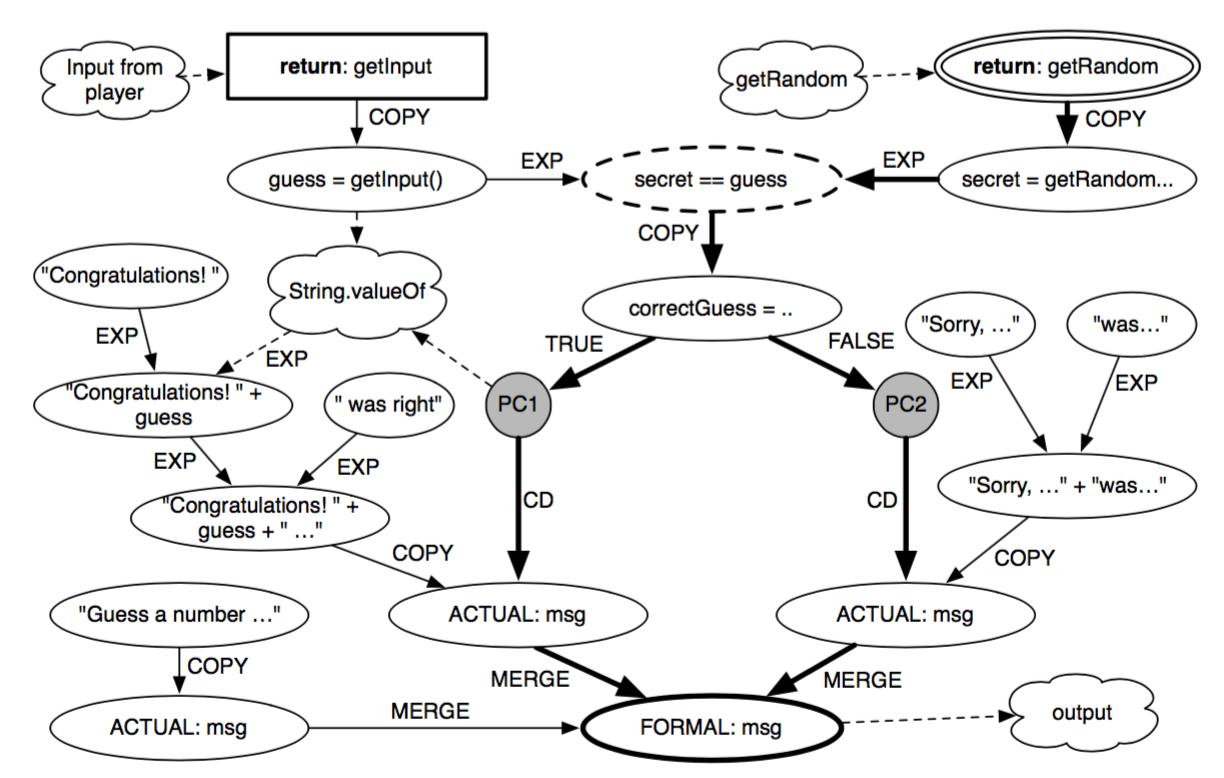
\includegraphics[width=0.7\textwidth]{images/PDG} 
      \caption{Program dependence graph of a guessing game}
    \label{fig:PDG}
\end{figure}

We can see that the value that flows to the output function indirectly depends on the value of the secret. This can be seen as a security violation and can be queried for in the Pigdin language. To this extent, the Pidgin Query Language (PidginQL) defines specialized constructs that allow the user to retrieve all relevant information from the PDG. As the program is represented as such a graph, the approach specializes in detecting if there is information flow from one node to another. An example of a PidginQL query is seen in listing \ref{lst:PidginExample}. The usual approach to writing queries goes as follows: First, the nodes between which information flow needs to be detected are specified and stored in variables. This is done through the aforementioned constructs. After specifying these \textit{source} and \textit{sink} nodes, another type of nodes can also be stored in a variable, namely \textit{declassifier} nodes. These nodes act as 'sanitizers' in a way that when information flows between a source and a sink and this information also flows through a sanitizer, then the flow is allowed. When all node have been captured in variables, declassifier nodes can be removed from the graph. The resulting graph is now modified in such a way that only the user-specified declassifier nodes are are removed. On this graph the final check is done if there is any flow left between the specified sources and sinks. 

\begin{lstlisting}[label={lst:PidginExample},language=JavaScript,caption=A typical PidginQL query,mathescape=true]  % float=t?

//source, sink and declassifier
let source = pgm.returnsOf("getRandom") in 			
let sink = pgm.formalsOf("output") in 				
let declassifier = pgm.forExpression("secret == guess") in
//Remove declassifiers and check for flow
pgm.removeNodes(declassifier).between(source, sink)	 		
is empty											
\end{lstlisting}

The PidginQL language is expressive and powerful for detecting information flows. The language however lacks expressiveness when it comes to inspecting nodes. There are no constructs that allow the user to only find nodes with a certain name, for example. A second limitation is the result of queries. Most static analysis tools report all found violations, with more information about the violating code. PidginQL on the other hand just indicates whether there is flow or not (remember the \texttt{is empty} construct on line 7).

\subsection*{Metal}

Metal\cite{Metal} can best be described as a general analysis tool of programs for which a user has to write application-specific extensions (also called checkers). These extentions are then executed as a traditional dataflow analysis, but can be augmented in ways outside the scope of traditional approaches. Metal extensions are applied depth-first to the control-flow graph of a function. This flow graph is computed from the AST of the program. By applying an extendion depth-first, each program point down a single path is checked. This process is very similar to pattern matching. Checkers in the Metal language consist of two parts: The actual code that describes the checker and a corresponding state machine. They distinguish two types of state machines: \textit{Global} state machines and \textit{variable-specific} state machines. The former detects program-wide properties, whereas the latter detects object-specific properties. 

Checkers are written by defining states between which the state machine can transition. When the current program point matches a pattern described in the current state of the checker, the state machine transitions to the next state and/or performs an action (usually printing a warning). When there is no match with the current program point, the state machine doesn't transition and the analysis continues with the next program point. Example \ref{fig:Metal} clarifies the approach. The example shows an global extension which checks for the double enabling of disabling of interrupts (\texttt{sti()} and \texttt{cli()} respectively). When enabling interrupts, the state machine transitions to the 'enabled' state. when then enabling interrupts again, an error showing "Double sti" is printed. The same happens for disabling interrupts: When a user attempts to disable interrupts twice, or when the end of a path is reached when interrupts are still disabled (and thus the state machine is still in the 'disabled' state), an error will be printed.

\begin{figure}[!ht]
    \centering
      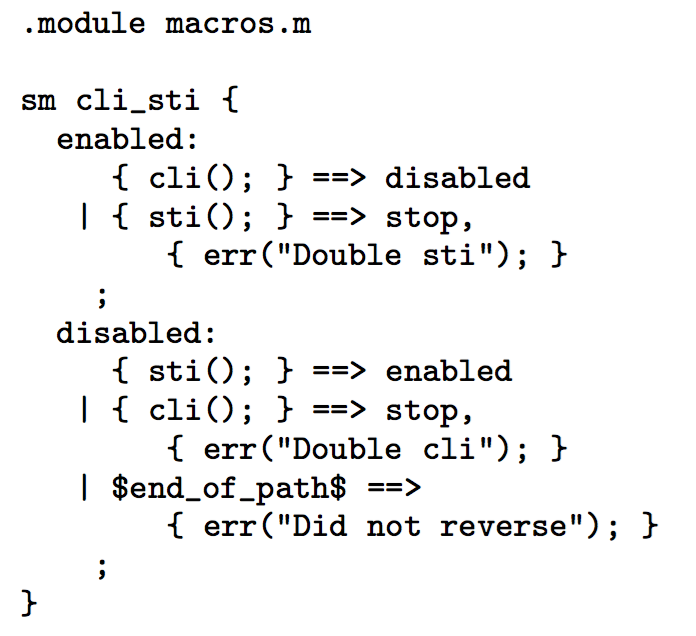
\includegraphics[width=0.5\textwidth]{images/Metal} 
      \caption{A simple double enabling/disabling checker}
    \label{fig:Metal}
\end{figure}

The Metal language is a good example of a clearly readable query language. Pattern matching languages are often most readable, and the approach used in Metal is both very expressive and flexible. Describing the states in the order one wishes to detect them is in our opinion the sweet spot between powerful, expressive languages and flexible, readable languages.

\subsection*{JunGL}

In contrast with other languages presented in this section, JunGL\cite{JunGL} is a scripting language to perform refactorings, based on pattern matching. The interesting part of their approach is how they specify which parts of the code they wish to refactor. In order to refactor some source code, the program first has to be represented in some way which is easy to access programmatically. They do this by parsing the code into a uniform graph, initially containing only the information of the parsed AST. Lazy edges containing control flow information can also be added to the graph, but only when the refactoring needs this information. JunGL makes use of \textit{path queries} to express which patterns they wish to match. We believe that these queries are both very readable and very expressive. For example, figure \ref{fig:JunGL} shows the path query to find the path from a variable occurence \texttt{var} to its declaration as a method parameter:

\begin{figure}[!ht]
    \centering
      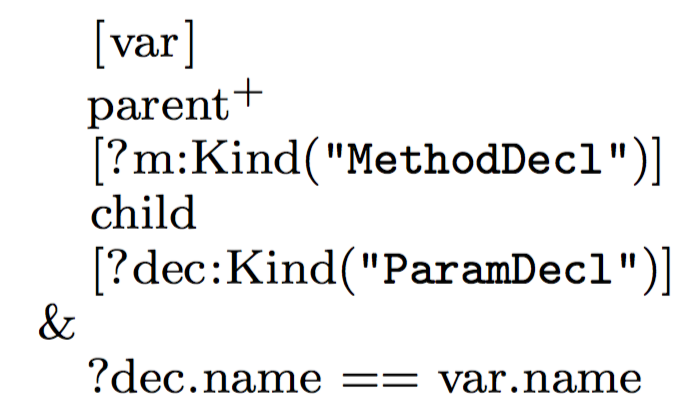
\includegraphics[width=0.4\textwidth]{images/JunGL} 
      \caption{A typical JunGL path query}
    \label{fig:JunGL}
\end{figure}

The above style of query denotation offers the exact amount of flexibility, readability and expressiveness that we need to let developers express user-specified queries over a graph. An additional advantage of this type of queries is that no boilerplate code is needed for writing queries, giving an 'out-of-the-box' feel to this type of languages.


\section{Conclusion}
In this chapter we discussed what static analysis is and why it is important for detecting characteristics and vulnerabilities in source code. We have also seen some approaches that enable users to write clean and readable queries that define the patterns to be detected. We can conclude that the state of the art in static analysis has reached a point where tools that support the detection of generic patterns often aren't expressive and flexible enough for application-specific use. A solution for this problem is a tool and a language which allow users to specify their own, custom queries for an application. In this way, no database of pre-encoded vulnerability detection queries is needed as the queries that are specified will mostly be too application-specific to generalize. We believe that expressing vulnerability queries (in the rest of this dissertation referred to as \textit{security policies}) is most readable and expressive using path expressions, as they can nearly be read as a regular sentence consisting of consecutive pieces of code/states to be detected.